\documentclass[10pt, a4paper]{scrreprt}

	% TODO: export in Layout-File
	% parse into new layout!
	% create table of bibliography
	% Schriftgröße, Seitenränder, Abstand erhöhen --> erst zum Schluss ;-)

%% --------------------------- LAYOUT ------------------ %%
\usepackage[T1]{fontenc}
\usepackage[utf8]{inputenc}
\usepackage[ngerman]{babel}
\usepackage{amsmath}
\usepackage{amssymb}
\usepackage{selinput}
\usepackage{setspace}
\usepackage{geometry}
\usepackage{graphicx}
\usepackage{makeidx}

\SelectInputMappings{
 adieresis={ä},
 germandbls={ß},
}
\setlength{\topskip}{\ht\strutbox} % behebt Warnung von geometry
\geometry{paper=a4paper,left=30mm,right=20mm,top=40mm} 
\graphicspath{{pictures/}} % Specifies the directory where pictures are stored
\makeindex

\onehalfspacing % Zeilenabstand erhöhen (1.5) 
% Seitenränder erhöhen!


%% ------------------------------------------------------ %%
%% ------------------------ BEGIN ---------------------- %%
%% -------------------------------------------------------%% 

\begin{document}


%% ---------------------------- TITLE ------------------------%%
\begin{titlepage}
\title{Implementierung einer Smartphone-Anwendung zum Austausch verschlüsselter Daten mit einer Cloud}
\maketitle
\end{titlepage}

% Text komplett in der Mitte von der Seite!
\vspace*{\fill}
\begin{center}
“If you think technology can solve your security problems, then you don’t understand the problems and you don’t understand the technology.”
\end{center}
\begin{flushright}
Bruce Schneier
\end{flushright}
\vspace*{\fill}


\tableofcontents

%% -------------------- EINLEITUNG ------------------ %%
\chapter{Einleitung}
% \setcounter{page}{1}
"Die Computer- und Internetnutzer in Deutschland setzen seit Bekanntwerden der geheimdienstlichen Abhöraktionen häufiger Verschlüsselungsverfahren ein." %[http://www.bitkom.org/files/documents/BITKOM-Presseinfo_Verschluesselung_18_12_2013_v2\%281\%29.pdf]
Aus der Pressemitteilung der BITKOM geht weiterhin hervor, dass von Juli 2013 auf November 2013 insgesamt 1,1 Millionen mehr Bundesbürger ihre persönlichen Dateien verschlüsseln. Besonders wichtig ist der Aspekt der Sicherheit, wenn es sich bei den Daten um relevante oder firmeninterne Informationen handelt, wie es z. B. am \index{Deutschen Elektronen Synchrotron (DESY)} in Hamburg der Fall ist. Auch der Austausch von Daten von mobilen Endgeräten wie \index{Smartphones} oder Tables spielen eine immer größere Rolle wie die Entwicklung der letzten Jahre zeigt (siehe Grafik). \\ 
\begin{center}
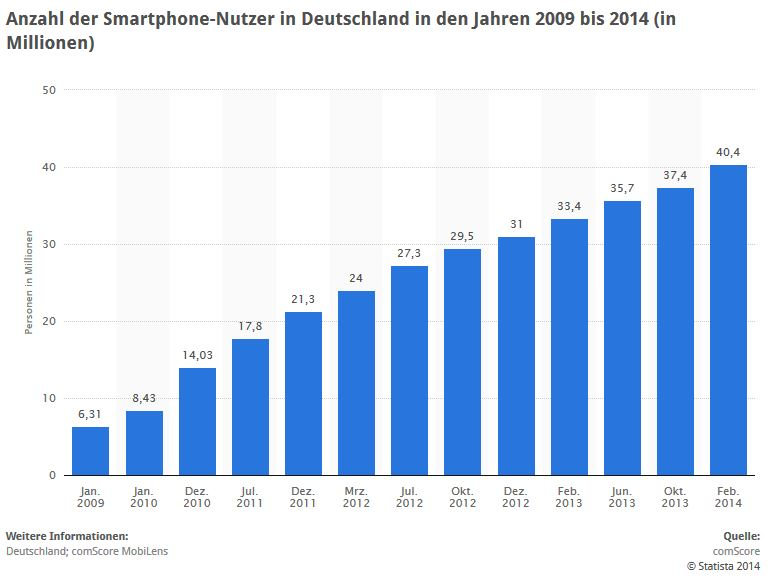
\includegraphics[scale=0.6]{smartphoneUser_Germany.JPG} %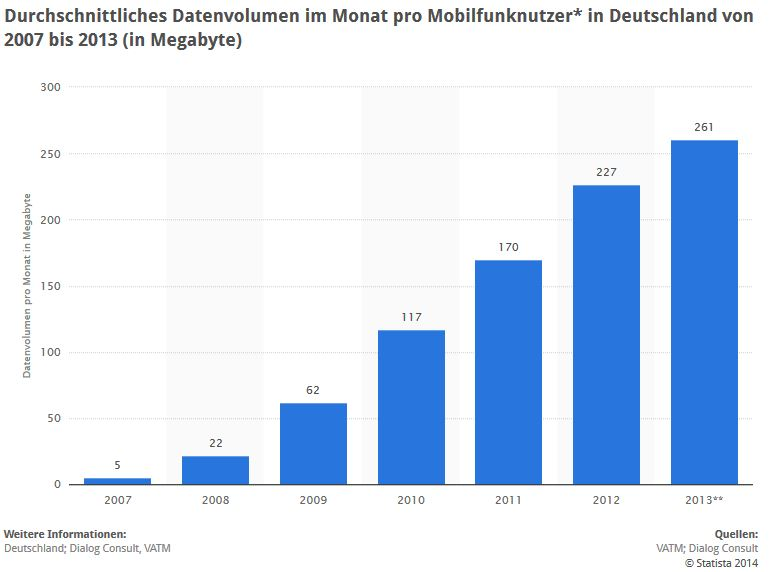
\includegraphics[scale=0.40]{datatraffic_germany.JPG} % zweite Grafik evtl. an anderer Stelle passender?
\end{center}
% http://de.statista.com/statistik/daten/studie/198959/umfrage/anzahl-der-smartphonenutzer-in-deutschland-seit-2010/
% http://de.statista.com/statistik/daten/studie/12885/umfrage/marktanteil-bei-smartphones-nach-betriebssystem-weltweit-seit-2009/
% http://de.statista.com/statistik/daten/studie/3506/umfrage/monatliches-datenvolumen-pro-mobilfunknutzer-in-deutschland/
Herkömmliche Verfahren zum Austausch von Daten reichen oftmals nicht mehr aus, wenn man den Aspekt der Sicherheit näher beleuchtet. % TODO: prüfen? kann man das so stehen lassen?!?


\section{Motivation}
Am Deutschen Elektronen Synchrotron, im folgenden DESY, werden bisher wichtige und sensible Dokumente über ein Programm Namens Dropbox gesichert und verwaltet. Dropbox bietet eine plattformunabhänginge Möglichkeit Dokumente Online abzuspeichern und von einem anderen Standort über ein internetfähiges Gerät wieder zu öffnen [https://www.dropbox.com/]. Auch wenn Dropbox nach eigenen Angaben den Advanced Encryption Standard (AES)  verwendet, bevor die Daten gespeichert werden, liegen die dafür notwendigen Schlüssel in Händen der Betreiber selbst, die somit vollen Klartextzugriff auf die Nutzerdateien haben. Dropbox begründet diesen Zugriff wie folgt:  "Wie die meisten Online-Dienste verfügt auch Dropbox über einen kleinen Mitarbeiterstamm, dem aus in unserer Datenschutzrichtlinie dargelegten Gründen Zugriffsrechte auf Nutzerdaten gewährt werden muss [...]". \\ % TODO [https://www.dropbox.com/help/27/de aufgerufen 01.07.2014]
Da das DESY über eine eigene Cloud-Infrastruktur verfügt, sollen in Zukunft alle wichtigen Daten nicht nur in dieser Cloud gespeichert werden, sondern auch zusätzlich durch eine Verschlüsselung gesichert werden. Die Cloud am DESY stellt im Hintergrund ein Rechnernetz zum Abspeichern von Daten zur Verfügung. Durch das Programm dCache, welches das Rechnernetz im Hintergrund steuert und verwaltet, ist es dem Anwender möglich Daten in das System zu speichern, ohne dessen Struktur zu kennen. dCache sorgt dafür dass die Daten, je nach Bedarf, mehrfach abgelegt werden und bei einem Zugriff schnell zur Verfügung stehen. Die Dateien selbst werden im Hintergrund auf verschiedene Datenträger, wie z. B. SSD-Festplatten, Magnetbänder, Tapes o. ä., abgelegt. Das System sorgt dafür, dass bei reger Anfrage die Daten, sofern möglich, auf ein schnelleres Medium repliziert werden. Die genaue Struktur und Vorgehensweise des Programmes ist jedoch nicht Teil dieser Arbeit, da das hier zu entwickelnde Programm nur die Schnittstelle des dCache-Servers verwendet.


\section{Zielsetzung}
Ziel dieser Arbeit ist es aus diesem Grund einen Prototyp zu entwickeln, der einerseits mit dem Cloud-System des DESY Kommunizieren kann um dort Dateien hoch- und herunter zu laden, andererseits diese Daten auch in angemessener Form (siehe Kapitel Validierung) zu Verschlüsseln. \\
In der ersten Version dieser Arbeit wird ein Programm entwickelt, welches auf Android-Betriebssystemen zum Einsatz kommen kann. Darüber hinaus ist es wichtig, dass die entsprechenden Schlüssel zum entschlüsseln der Daten nicht zusammen mit den Daten abgelegt werden, sondern ausschließlich den Parteien des Datenaustauschs bekannt sein soll. Dies bedeutet, das selbst die Betreiber am DESY nicht die Möglichkeit haben die abgelegten Daten zu entschlüsseln. \\
Zum Ver- und Entschüsseln der Daten sollen Verfahren verwendet werden, die in der heutigen Zeit als sicher angesehen werden und Smartphones im Bezug auf Performance und Akkuverbrauch nicht zu stark belasten. Um diese Faktoren zu Validieren wird eine Testanwendung geschrieben, die mit bestimmten Faktoren die verschiedenen Verfahren untereinander überprüfen (siehe Kapitel Validierung).

	% TODO: Prüfen, ob dieser Part wirklich hier rein muss? Andere Software vergleichen?
\section{Verwandte Arbeiten}
	% TODO: Recherche?!? --> wird nicht benötigt, da es sich bei der Arbeit hautpsächlich um die Entwicklung des Programmes handelt. Kryptographische Verfahren wurdne zu genüge behandelt.
\section{Verwandte Programme}
	% TODO: Unterscheidung in Arbeiten & Programme notwendig?
	% vgl. Dropbox
	% vgl. ownCloud <<- speziell: soll in Zukunft am DESY verwendet werden --> kompatiblität beachten?!? 
	% vgl. boxcryptor
	% vgl. cloudfogger


\section{Diese Arbeit}
\subsection{Inhaltlicher Aufbau}

% \chapter{Anforderungen} ?


%% ---------------------- GRUNDLAGEN ----------------- %%
\chapter{Grundlagen Android}
Android ist ein Betriebssystem für Smartphones und Tablets, welches von der open handset alliance entwickelt wird. Das Konsortium besteht aktuell aus 84 Unternehmen, die an der Entwicklung des Betriebssystems arbeiten. %http://www.openhandsetalliance.com/index.html]
In diesem Kapitel wird kurz darauf eingegangen, welche Kryptografischen Aspekte Android in den verschiedenen Versionen zur Verfügung stellt um diese im darauffolgenden Kapitel genauer zu Untersuchen. Aufgrund der Tatsache, dass die Android Version Gingerbread (2.3.3) im Juni 2014 noch einen Marktanteil von knapp 15\% hält, ist dies auch die niedrigste vom Programm unterstützte Version. \\
\begin{center}
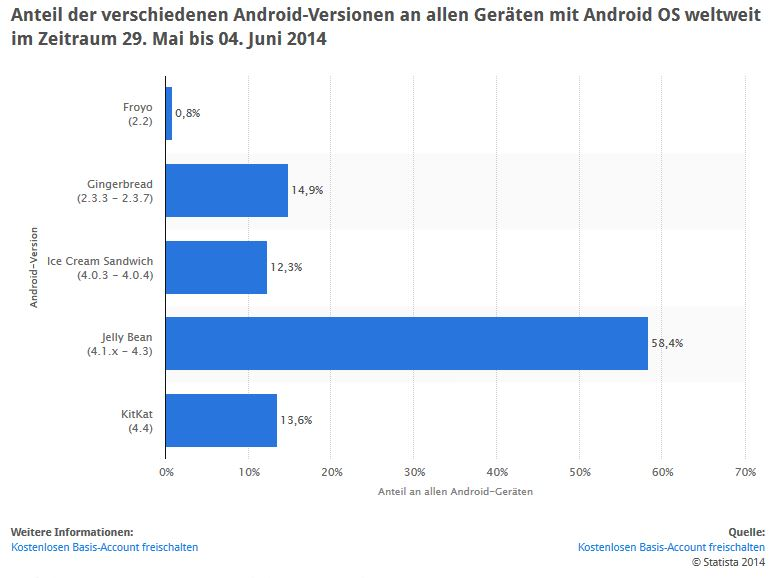
\includegraphics[scale=0.6]{android_version_marktanteil.JPG} %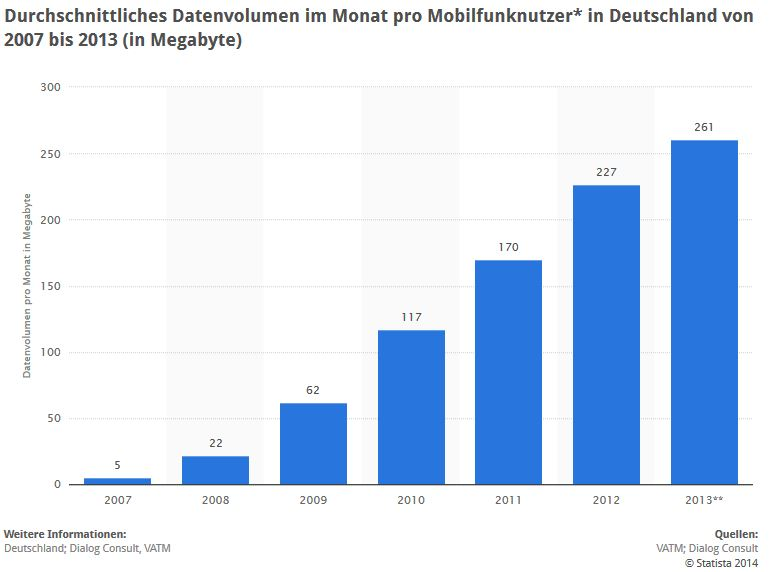
\includegraphics[scale=0.40]{datatraffic_germany.JPG} % zweite Grafik evtl. an anderer Stelle passender?
\end{center}
Bei der Analyse wird darauf geachtet, dass alle Funktionalitäten die im Programm entwickelt werden, von dieser Version unterstützt werden. Die, während des Schreibens dieser Arbeit, aktuellste Version der Android API ist KitKat (4.4), bei der darauf geachtet wird, dass die eingesetzten Funktionen auch in dieser Version noch zur Verfügung stehen und nicht mit \textit{deprecated (veraltet)} markiert sind.


\section{Zusammenhang Kryptographie}
Beim Thema Sicherheit im Zusammenhang mit Android ist erstmals der Begriff der Sandbox zu nennen. Eine Anwendung wird abgekapselt in einer eigenen Umgebung mit eigenem Prozess, eigenem Betriebssystem-User, eigener Dalvik-VM, eigenem Heap und eigenem Dateisystem ausgeführt. Dieses abgekapselte Konstrukt wird Sandbox bezeichnet. Dadurch ist es dem Betriebssystem möglich unerlaubten Zugriff auf Ressourcen oder andere Programme zu beschränken, hierbei wird das Berechtigung- und Prozess-Management-System von Linux verwendet. %Becker, Arno Android 4.4 - Seite 33]
Um dennoch verschiedene Zugriffe zu erlauben muss in der sogenannten Manifest-Datei der Anwendung die Berechtigung festgelegt und vom Benutzer bei der Erstinstallation bestätigt werden.
Auch wenn dieses Konzept Daten zur Laufzeit innerhalb einer Anwendung schützt, ist es möglich Dateien auch auf einer SD-Karte zu speichern, in das Internet zu verschicken oder über andere Wege auszutauschen. Diese Daten sind dann außerhalb der Anwendung und gegen externe Zugriffe nicht mehr geschützt.
Dennoch gibt es die Möglichkeit in Android diese Daten zusätzlich mit einer Verschlüsselung zu versehen - hierfür stellt Java, seit der Version 1.4, die \textit{Java Cryptography Extension (JCE)} innerhalb von Android zur Verfügung. Innerhalb der Erweiterung (engl. extension) sind verschiedene Provider eingebunden, die dem Programmierer die Möglichkeit geben Kryptografische Verfahren aufzurufen, ohne die genaue Implementierung kennen zu müssen. In Java-Anwendungen gibt es diverse Implementierungen von Sun, die jedoch aus Datenschutzrechtlichen Gründen nicht in der Android Java-API vorhanden sind. der Provider Bouncy-Castle stellt eine Alternative zur Implementierung von Sun darf und wird in Android zur Verfügung gestellt. Innerhalb von Android wurde das Paket so geändert, dass es den Richtlinien der JCE entspricht. 
Bouncy-Castle ist einer der von Android zur Verfügung gestellten Provider - jedoch gibt es noch weitere Provider, die selbige oder andere Implementierungen zur Verfügung stellen. Mit folgendem Codeabschnitt ist es möglich die einzelnen Provider mit den unterstützten Verfahren auszulesen und untereinander zu vergleichen. Dieser Code wurde auf verschiedenen Versionen ausgeführt, um die Unterschiede der einzelnen Versionen hervorzuheben. \\
\begin{center}
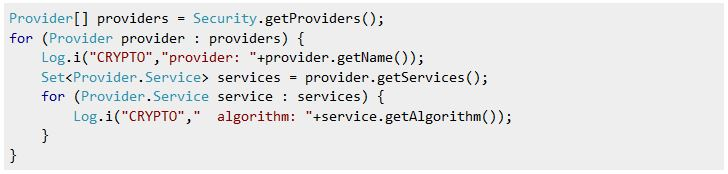
\includegraphics[scale=0.8]{read_cryptoprovider.JPG} %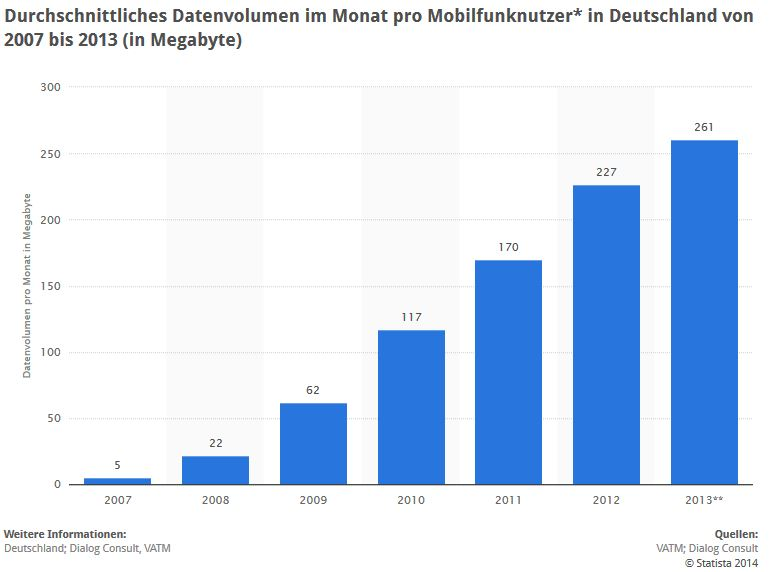
\includegraphics[scale=0.40]{datatraffic_germany.JPG} % zweite Grafik evtl. an anderer Stelle passender?
\end{center}
Im Vergleich stehen folgende Android-Versionen:
\shorthandoff{"}
\begin{itemize}
\item 2.3.3 (Gingerbread) : die niedrigste vom Programm unterstützte Version
\item 4.1.1 (Jelly Bean) : die Version des Entwickler-Gerätes
\item 4.4.4 (KitKat) : aktuellste auf dem Markt verfügbare Android-Version
\item "L" : zukünftige Version, welche bereits zu Testzwecken als Entwickler-Version freigeschaltet ist. Der Codename "L" zeigt auf, dass es sich in der Folge der Süßigkeiten (Gingerbread, HoneyComb, Ice Cream Sandwich, Jelly Bean, KitKat) vermutlich alphabetisch fortsetzen wird - die Versionsnummer ist bis dato nicht bekannt.
\end{itemize}
Im Vergleich der Ausgabe eines Gerätes mit Android 2.3.3 und eines mit 4.1.1 bzw. 4.4.4 und "L" liegt der Hauptunterschied in der Unterstützung von Elliptischen Kurven für das Diffie-Hellmann-Verfahren (ECDH) und den Digital-Signature-Algorithm (ECDSA), welche in der Version 2.3.3 nicht unterstützt werden. Des Weiteren ist ab der Version 4.4.x der Provider OpenSSL und deren Algorithmen spezifischer dargestellt.
Folgende Verschlüsselungsverfahren werden sowohl von der Version 2.3.3 als auch von der Version 4.1.1 , 4.4.4 und L unterstützt und werden im nachfolgenden Kapitel näher erläutert: \\ \\
\begin{tabular}{|l|l|} \hline\hline
\textbf{Verschluesselung} & \textbf{Hash-Funktion} \\ \hline &  \\
AES & MD5 \\
ARC4 & SHA1 \\
Blowfish & SHA256 \\
DES & SHA384 \\
3DES & SHA512 \\
RSA & \\
ElGamal & \\
\hline\hline
\end{tabular} \\
\\Des Weiteren wird das Key-Wrap-Verfahren (AES und 3DES), der Authentifizierungsalgorithmus HMAC und der Standard X509 beschrieben. Die Vollständige Liste aller Unterstützen Algorithmen mit dessen Providern befindet sich im Anhang. Welcher Provider für welchen Algorithmus besser geeignet ist, kann man nicht pauschalisieren und auch nicht auf einen spezifischen Anwendungsfall verallgemeinern. Im Kapitel Validierung werden Geschwindigkeitsaspekte beider großen Provider (OpenSSL und Bouncy-Castle), sofern möglich, gegenübergestellt um für jeden Algorithmus den geeigneten Provider zu wählen. Falls es innerhalb eines Providers zu größeren Sicherheitslücken von einem verwendeten Algorithmus kommt, ist es durch das JCE möglich diesen ohne weitere Code-Änderungen zu wechseln. 


\chapter{Grundlagen Kryptologie}
Das Wort Kryptologie stammt aus dem Griechischen \textit{kryptós} für verstecken und \textit{lógos} für die Lehre.% [Duden http://www.duden.de/rechtschreibung/krypto_, http://www.duden.de/rechtschreibung/_logie] 
Dieser Zweig umfasst die Kryptographie - die Wissenschaft die sich mit der Absicherung von Daten beschäftigt, die Kryptoanalyse - welche für das Aufbrechen von Geheimnachrichten zuständig ist sowie der Mathematik.
Im Bereich der Kryptologie ist es das Ziel eine Nachricht, welche aus lesbaren Zeichen (Klartext) besteht unverständlich zu machen (Verschlüsseln) und daraus einen Geheimtext (Chiffretext) zu erzeugen. Dieses Verfahren wird mit mathematischen Funktionen und einem Schlüssel (Key) durchgeführt. Die Umkehrung von Chiffretext in Klartext (Entschlüsselung) wird ebenfalls durch eine mathematische Funktion und einen Schlüssel durchgeführt. Ziel dieser Ver- und Entschlüsselung ist es Nachrichten zwischen einem Sender und Empfänger so auszutauschen, dass ein Angreifer diese nicht mitlesen, oder im verschärftem Sinne nicht verändern kann. Hierbei besteht eine Nachricht in der Informatik immer aus binären Daten und kann eine Textdatei, ein Bild, ein Video oder vieles mehr darstellen. Ver- und Entschlüsselung sind mathematische Funktionen, die auf den Klartext, bzw. auf den Chiffretext angewendet werden. 


\subsubsection{Terminologie}
Um die Lesbarkeit zu erhöhen wird Klartext im folgenden mit M (engl. Message), Chiffretext mit C (engl. Chiffre), die Verschlüsselungsfunktion mit E (engl. Encoding), die Entschlüsselungsfunktion mit D (engl. Decoding) und dem Schlüssel K (engl. Key) beschrieben.
Zum Verschlüsseln kommt also folgende Funktion zum Einsatz: \\ \\
E$_{K}$(M) = C\\ \\ 
Um den Chiffretext wieder zu Entschlüsseln wird die umgekehrte Richtung angewandt:\\ \\
D$_{K}$(C) = M\\ \\
Zusammengefasst muss also gelten: das Verschlüsseln einer Nachricht und das darauffolgende Entschlüsseln des erzeugten Chiffretextes, mit der dazugehörigen Funktion und korrektem Schlüssel, muss wieder den Klartext ergeben. Mathematisch beschrieben ist das wie folgt:\\ \\
D$_{K}$(E$_{K}$(M)) = M\\ \\
Um einen sicheren Kanal zwischen Sender und Empfänger zu gewährleistet, reicht es nicht allein die Nachricht zu verschlüsseln. Authentifizierung, Integrität und Verbindlichkeit müssen darüber hinaus gewährleistet sein um sicher zu Kommunizieren. \\ \\
\textbf{Authentifizierung} beschreibt hierbei das Verfahren indem sich die Identität einer Person beweisen lässt. Im Umkehrschluss bedeutet das, dass sich ein Angreifer nicht als eine andere Person ausgeben kann. Aus der Authentifizierung folgt dann die \textbf{Autorisierung}, also das Prüfen, ob der Benutzer die Rechte hat, die er fordert.\\ \\
\textbf{Integrität} bedeutet, dass sichergestellt werden kann, dass eine Nachricht bei der Übermittlung zwischen Sender und Empfänger nicht durch einen Angreifer verändert wurden ist. \\ \\
\textbf{Verbindlichkeit} beschreibt  dass der Sender nicht leugnen kann, dass eine Nachricht gesendet wurde. Dies ist eine Steigerung der Authentifizierung, denn durch Verbindlichkeit ist es außerdem gewährleistet, dass der Empfänger einer Nachricht gegenüber einer dritten Person den Absender der Nachricht glaubwürdig machen kann.\\ \\


\subsubsection{Kerhoff's Maxime}
Ein Aspekt in der Kryptographie sind die Kerkhoffs' Maxime, die folgendes Aussagen: "the security of the encryption scheme must depend only on the secrecy of the Key K$_{e}$, and not on the secrecy of the algorithms." [Schneier, 1997] Übersetzt bedeutet es, dass die Sicherheit eines Kryptographischen Verfahrens  auf der Geheimhaltung des Schlüssels beruhen muss und nicht auf derer des Verschlüsselungsalgorithmus.


\subsubsection{Verfahren}
Prinzipiell unterteilt man Kryptographie in zwei Verschiedene Verfahren. Die symmetrischen Verfahren und die asymmetrischen, auch public key infrastructure genannt. Generell lässt sich über das "bessere Verfahren" keine Aussage treffen, da es für beide Verfahren Vor- und Nachteile gibt. Bruce Schneier fasste es wie folgt zusammen: \\
"Symmetrische Kryptographie eignet sich am besten zur Verschlüsselung von Daten. Sie ist um Größenordnungen schneller und nicht anfällig für chosen-ciphertext-Angriffe. Public-Key-Kryptographie schafft Dinge, die außerhalb des Einsatzbereichs symmetrischer Kryptographie liegen und eignen sich am besten für die Schlüsselverwaltung und eine Vielzahl der Protokolle [...]."\\ %[Schneier, 1996 übersetzt, Seite 254f]
Der im Zitat verwendete Ausdruck, chosen-ciphertext-Angriff beschreibt einen Angriff auf ein Kryptosystem, bei dem der Kryptoanalytiker verschiedene Chiffretexte zur Entschlüsselung auswählen kann und entsprechend Zugriff auf den dazugehörigen Klartext besitzt. Die Aufgabe bei dieser Art des Angriffes besteht darin, den entsprechenden Schlüssel herauszufinden. %[Schneier 1997, Seite 7]
Neben der chosen-ciphertext-Angriffe gibt es weitere Angriffsszenarien auf Kryptosysteme, wie z. B. ciphertext-only, known-plaintext, chosen-plaintext, chosen-key und weitere. Da es sich bei dieser Arbeit nicht um eine Kryptoanalyse eines Systems handelt, werden diese Szenarien nicht näher erläutert. Es wird davon ausgegangen, dass wenn eines dieser Szenarien zum knacken des Systems führt, dieses kryptographische Verfahren bereits heute als unsicher angesehen wird.


\section{Symmetrische Verfahren}
Bei symmetrischen Verschlüsselungsverfahren existiert ein Schlüssel, der jeweils für Ver- und Entschlüsselung verwendet wird. Dieser Schlüssel muss bereits beiden Parteien bekannt sein, bevor ein verschlüsselter Kanal aufgebaut werden kann. Eines der Probleme bei symmetrischen Verfahren ist der Austausch des Schlüssels, den man von Sender zu Empfänger, bereits vor der sicheren Kommunikation, übertragen muss (siehe Kapitel Schlüsselvereinbarung). Symmetrische Verfahren unterteilt man in zwei Grundtypen, die Block- und Stromchiffrierung. Bei der Blockchiffrierung wird der Klartext in Blöcke, mit fester Größe, aufgeteilt und innerhalb des Blockes werden die mathematischen Funktionen angewandt. Bei der Stromchiffrierung werden die Daten nicht in Blöcken zusammengefasst, sondern jedes einzelne Klartextbit wird in ein Chiffrebit überführt. [Schneier 1996, Seite 223] 

\subsection{Betriebsmodi}
Betriebsmodi sind verfahren bei der das eigentliche Kryptografische Verfahren mit einer Rückkopplung und einigen einfachen Operationen verknüpft wird. Ist eine Nachricht länger als die für das Verfahren angegebene Blocklänge, so muss die Nachricht mit einem Betriebsmodi angepasst werden. Wichtig bei den verschiedenen Betriebsmodis ist, dass sie die Sicherheit des Cryptoverfahrens nicht beeinträchtigen.

\subsubsection{Padding}
Bei der Blockchiffrierung ist eine fest Blocklänge vorgegeben, in der die Daten vorhanden sein müssen. Ist dies nicht der Fall, müssen diese so modifiziert werden, dass das Verfahren damit umgehen kann.
Um z. B. den letzten Block einer Nachricht, der nicht der Blocklänge entspricht, zu vervollständigen wird er mit einem regelmäßigen Muster aufgefüllt. Das Muster und die Art dieser Auffüllen, bzw. das Kennzeichnen hängt von den Verschiedenen Padding-Verfahren ab. (z. B. PKCS5, PKCS7 o. ä.)

\subsubsection{ECB}
ECB (\textit{electronic codebook mode}) ist ein Betriebsmodi, bei der der Klartext in verschiedene Blöcke, der benötigten Länge, aufgeteilt wird und jeder dieser Blöcke einzeln verschlüsselt werden. Das Konkatinieren dieser Blöcke ergibt dann den neuen Chiffretext. Problem bei diesem Verfahren ist, dass 2 gleiche Klartextblöcke auf den identischen Chiffreblock ergeben, was wiederum für den Angreifer sichtbar und Nutzbar sein kann. Aus diesem Grund wird ECB als unsicher angesehen und sollte deshalb nicht verwendet werden (Do not ever use ECB for anything [Ferguson 2003, Seite 69]).

\subsubsection{CBC}
Beim \textit{cipher block chaining mode} (CBC) wird das Problem von ECB umgangen, indem man jeden Klartextblock mit den vorherigen Chiffretextblock mit einer XOR-Verknüpfung durchführt: \\ \\
C$_{i}$ = E(K, P$_{i}$ $\oplus$ C$_{i-1}$) \\ \\
Dadurch werden alle Bits eines Klartextblockes mit einer bereits verschlüsselten Nachricht verknüpft. Gleiche Blöcke werden so mit unterschiedlichen Cryptotexten verknüpft und ergeben so unterschiedliche Ausgaben.
Da die obenstehende Formel erst angewandt werden kann, wenn ein Chiffretextblock vorliegt muss die Möglichkeit geschaffen werden, den ersten Klartextblock auch zu verknüpfen (also C$_{0}$). Der Initiale Block der für diese Verknüpfung angewandt wird heißt \textit{initialization vector} (IV).
Es gibt verschiedene Möglichkeiten diesen initialization vector zu bestimmen. Zum einen kann man einen festen IV für alle Nachrichten wählen, das hätte wiederum zur Folge, dass 2 gleiche Klartextblöcke zu einem identischen Chiffreblock verschlüsselt werden (siehe ECB). Als weitere Möglichkeit besteht den IV zu iterieren - jedoch ist auch diese Möglichkeit nicht zu nutzen, da sich der IV bei einer Iteration zu Beginn nur um 1 Bit unterscheidet und dies sich im Chiffretext dann auch lediglich auf 1 Bit auswirkt. Um alle Bits des ersten Klartextblocks zu verändert, besteht die Möglichkeit des sogenannten \textit{random IV}. Der Initialisierungsvektor wird komplett zufällig gewählt und entsprechend der Nachricht angehangen, oder vorangestellt, damit beim Entschlüsseln diese Verknüpfung wieder rückgängig gemacht werden kann.

\subsubsection{OFB}
Beim OFB (\textit{Output feedback mode}) wird nicht die Klartextnachricht zur Verschlüsselung benutzt, sondern eine Zufallsreihe von Bytes. Die daraus resultierende verschlüsselte Nachricht kann dann mit der Klartextnachricht verknüpft werden. Der Vorteil besteht darin, dass die Berechnung des Chiffretextes aus der Zufallsreihe bereits durchgeführt werden kann, bevor der eigentliche Klartext zur Verfügung steht. Dieses Verfahren ist außerdem in der Lage, Klartexte zu verschlüsseln die kleiner als die eigentliche Blocklänge sind (Wichtig für Byteweise Anwendungen, z. B. Terminalanwendungen). \\ \\
K$_{0}$ := IV \\
K$_{i}$ := E(K, K$_{i-1}$) \\
C$_{i}$ := P$_{i}$ $\oplus$ K$_{i}$ \\ \\



\subsubsection{CFB}
Der \textit{cipher feedback mode} ähnelt dem oben beschriebenen OFB Modus, mit dem Unterschied, dass die verschlüsselte Nachricht (nach Verknüpfung des Klartextes) als neuer Block für die nächste Verschlüsselung angesehen wird. Das bedeutet, dass eine Verschlüsselung erst stattfinden kann, sobald der erste Klartextblock vorliegt (Dieser kann, wie auch bei OFB, kleiner sein als die Blockgröße des zu Grunde liegenden Kryptoverfahrens). \\ \\
C$_{0}$ = P$_{0}$ $\oplus$ E$_{K}$(IV) \\
C$_{i}$ = P$_{i}$ $\oplus$ E$_{K}$(C$_{i-1}$) \\
P$_{i}$ = C$_{i}$ $\oplus$ E$_{K}$(C$_{i-1}$) \\

\subsubsection{CTR}
Im Counter-Modus kann die Berechnung des Schlüssels, wie auch beim OFB, vor dem ersten Klartextblock erfolgen. Innerhalb des Modi gibt es einen internen Zähler, der immer konstant erhöht wird. Aus diesem Zähler und dem Schlüssel wird dann ein neuer Schlüssel erzeugt, mit dem der Klartext verschlüsselt werden kann. Der Vorteil dieses Verfahrens besteht darin, dass man nicht die komplette Nachricht entschlüsseln muss, sondern einzelne Teile des Chiffretextes entschlüsseln kann. Hierfür setzt man den internen Zähler auf die gewünscht Stelle, erzeugt den Schlüssel und entschlüsselt den Chiffreblock. Wichtig ist, dass der selbe Zähler mit den selben Schlüssel nicht doppelt verwendet werden soll (Problem ECB: zwei identische Klartextblöcke ergeben identischen Chiffretext).

\subsection{DES, 3DES}
"Its restricted key size of 56 bits and small block size of 64 bits make it unsuitable for today`s fast computers and large amounts of data. It survives in the form of 3DES, which is a block cipher built from three DES encryptions in sequence. This solves the most immediate problem of the small key size, but there is no known fix for the small block size. [...] we do not recommend using either DES oder 3DES in new designs." [Ferguson 2003, Seite 51]
Niels Ferguson weißt darauf hin, dass DES aufgrund seiner Schlüsselänge von 56 bits und der Blockgröße von 64 bits ungeeignet für heutige Systeme ist. Weiterhin beschreibt er, dass auch durch 3DES das Problem der geringen Blockgröße nicht behoben wird und er schlussfolgert dass man in heutigen neuen Systemen beide Verfahren nicht verwenden sollte. \\
Da das System als unsicher angesehen ist, wird auf eine nähere Untersuchung und Erläuterung der mathematischen Funktionen verzichtet. DES und 3DES wird in der zu entwickelnden Anwendung nicht implementiert.

\subsection{AES}
Der Advanced Encryption Standard, im folgenden AES genannt, ist ein Verschlüsselungsverfahren welches auf Blockchiffrierung beruht und seit 2002 ein offizieller Standard ist. Entwickelt wurde der neue Standard mit dem Namen Rijndael bei einer Ausschreibung für einen neuen Sicherheitsstandard durch J. Daemen und V. Rijmen, die sich gegen 14 andere Konkurrenten durchsetzen konnten. Auch unter den besten 5 dieser Ausschreibung waren die Verfahren MARS, RC6, Serpent und Twofish, wobei keiner dieser fünf eine Sicherheitsschwäche aufwies. Rijndael konnte letztendlich durch seine einfache Struktur und gute Performance im Software-, sowie im Hardwarebereich überzeugen. %[Eckert 2012, Seite 343f]
Darüber hinaus hat die US National Security Agency (NSA) AES für interne Dokumente bis zum Sicherheitsstatus TOP SECRET, mit einer Schlüssellänge von 192 oder 256 und für den Sicherheitsstatus SECRET mit einer Schlüsselänge von 128 Bit erlaubt, was verdeutlicht, dass selbst Kryptographen von Geheimdiensten diesen Standard als sicher ansehen. %[http://wiki.crypto.rub.de/Buch/download/Understanding-Cryptography-Chapter4.pdf]


\subsubsection{Funktionsweise}
AES arbeitet mit einer Blockgröße von 128 Bit, also 16 Byte welcher intern als 2-Dimensionale Matrix (4x4) abgespeichert wird und auf der mathematische Funktionen angewandt werden.
Alle Funktionen innerhalb von AES werden Byteweise ausgeführt (8 Bit-Blöcke).  Die interne Nachricht bezeichnet man als \textit{state}, also den aktuellen Status des Blockes. \\
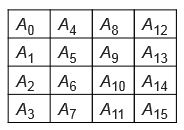
\includegraphics[scale=0.5]{aes_state.JPG} \\
Die Schlüssellänge des Verfahren ist entweder 128, 192 oder 256 Bit, wovon auch die auszuführende Rundenzahl abhängt (10 Runden bei 128 Bit, 12 bei 192 und 14 bei 256 Bit Schlüssellänge). In jeder dieser Runden werden Verfahren angewandt um den Klartext weiter zu verschlüsseln. Bei AES sind das \textit{ByteSubstitution, ShiftRow, MixColumns} und \textit{KeyAddition}. \\ \\
Ausgenommen von dieser Regel ist die letzte Runde, in der MixColumns ausgelassen wird. %[Eckert, Seite 345] 
Zusätzlich wird vor der ersten Runde die Funktion KeyAddition angewendet. %[http://wiki.crypto.rub.de/Buch/download/Understanding-Cryptography-Chapter4.pdf]


\subsubsection{ByteSubstitution}
In der Funktion ByteSubstitution wird eines der beiden Verfahren zum Verbergen von Redundanz angewendet - die Konfusion. Die Konfusion sorgt dafür, dass der Zusammenhang zwischen Klartext und Chiffrat verschleiert wird und möglichst aus einer kleiner Änderung im Klartext eine große Änderung im Chiffrat erzeugt wird. Hierzu wird jedes Byte in eine sogenannte S-Box eingegeben, wobei diese  wiederum ein Byte aus Ausgabewert hat (Dieses Verfahren wird für alle 16 Byte eines Blockes angewandt). Die S-Box selbst ist eine 16x16 Matrix, mit der zu jeder eingegebenen Bit-Reihenfolge eine neue Ausgabe-Reihenfolge erzeugt wird. Ziel ist es, durch minimale Veränderung des Eingabewertes eine maximale Veränderung des Ausgabewertes zu erzeugen. Darüber hinaus ist die in AES verwendete S-Box nicht linear - das bedeutet, dass die Addition zweier einzelner Ausgabewerte nicht das selbe Ergebnis liefert wie die Addition zweier Eingabewerte:\\ \\
\(S(A) + S(B) \neq S(A+B)\) \\ \\
Zusätzlich ist die S-Box bijektiv, es existiert also zu jeder Bitreihenfolge genaue eine eindeutige Zuweisung - Bitreihenfolgen die zwei Ausgabewerte erzeugen können existieren nicht. Im Umkehrschluss bedeutet das, dass jedes Ausgabebyte der S-Box wieder durch eine inverse S-Box zurück transformiert werden kann (Wird bei der Entschlüsselung verwendet). Die S-Boxen innerhalb von AES sind alle identische, sodass 16x pro Runde immer die selbe Matrix verwendet wird. Das hat zur Folge, dass sie in den den meisten Softwareimplementierungen durch fixe Tabellen realisiert werden, anstatt sie jedes mal neu zu Berechnen. Die Berechnung einer S-Box erfolgt durch Endliche Körper und eine fixe Multiplikation und Addition um die Logik der endlichen Körper zu verwischen. [c. Paar, Seite 102 %http://wiki.crypto.rub.de/Buch/download/Understanding-Cryptography-Chapter4.pdf]


\subsubsection{ShiftRow}
Das zweite Verfahren zum Vergeben von Redundanz ist die Diffusion, bei der die Redundanz verteilt wird (Einfachster Anwendungsfall ist das Vertauschen der Klartextbuchstaben in eine neue Reihenfolge). Eine Funktion die innerhalb von AES die für Diffusion sorgt, ist das ShiftRow-Verfahren. Hierbei werden die Bytes innerhalb einer Spalte des state-Blockes auf alle anderen Spalten aufgeteilt. Eine Änderung innerhalb einer Spalte (A$_{0}$ bis A$_{3}$ der state-Matrix) hat somit Auswirkung auf alle anderen Spalten (Auswirkung auf komplette State-Matrix). Folgende Grafik soll das verdeutlichen, wobei B$_{0}$, B$_{1}$, ..., B$_{15}$ jeweils die Bytes A$_{0}$, A$_{1}$, ..., A$_{15}$ nach der Transformation durch die S-Box sind. In der Grafik ist die interne 4x4 Matrix (state) hier Spaltenweise nebeneinander abgebildet. (Vergleiche state-Matrix)  \\ \\%TODO: Grafik-Nummer
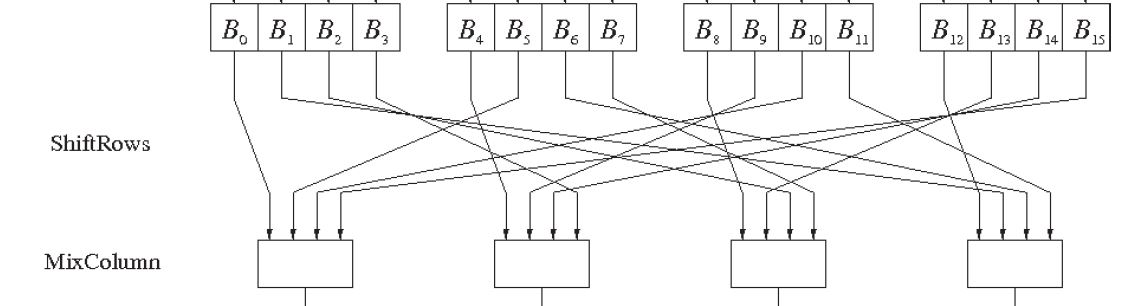
\includegraphics[scale=0.5]{aes_Shift_Row.JPG} \\ \\
Die in der Grafik gezeigten Linien, die die Verschiebung darstellen sollen, ist innerhalb der state-Matrix durch einfaches Shifting realisiert. Hierbei wird in der ersten Zeile keine Verschiebung durchgeführt, in der zweiten Zeile wird jedes Byte um 1 nach Links rotiert, in der dritten 2 nach Links und in der vierten Zeile 3 nach Links. \\ \\
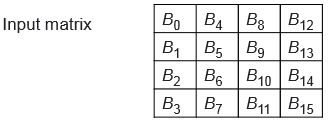
\includegraphics[scale=0.5]{shift_row_before.JPG}
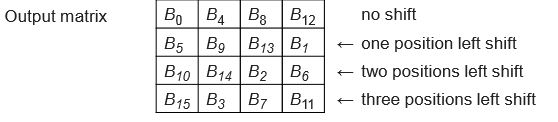
\includegraphics[scale=0.5]{shift_row_after.JPG} \\


\subsubsection{MixColumns}
Die MixColumns-Funktion ist die zweite Funktion in AES die für die Diffusion sorgt - sie bewirkt, dass die Änderung eines einzigen Eingabebytes in die Funktion alle Ausgabebytes verändert. Hierbei wird jede Spalte (als Vector dargestellt) mit einer festen 4x4 Matrix multipliziert. \\ \\
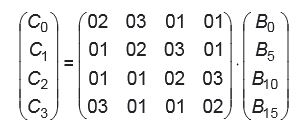
\includegraphics[scale=0.5]{aes_mixcol.JPG} \\
In der Grafik beschreibt der Vector B$_{0}$, B$_{5}$, B$_{10}$, B$_{15}$ genau die erste Spalte nach der Verschiebung durch ShiftRow. 
Durch die starke Diffusion die durch die Verteilung der Bytes von einer Spalte auf alle Spalten in der Funktion ShiftRow und die Vermischung aller Bytes durch die MixColumns-Funktion erreicht wird, ist es dem Verfahren AES mögilch in 3 Runden jedes Byte des Klartextes von allen 16Byte der state-Matrix abhängig zu machen. Wenn also die zu verschlüsselnde Nachricht aus einer 1 und restlichen Nullen besteht wird diese 1 in nur 3 Runden auf alle anderen Nullen Auswirkung zeigen.


\subsubsection{KeyAddition}
Beim KeyAddition wird jeweils der aktuelle Block (4x4 state-Matrix) mit dem aktuellen Rundenschlüssel (16 byte) via XOR Bitweise verknüpft. 

\subsubsection{Rundenschlüssel}
AES erzeugt für die verschiedenen Runden, die bei der Ver- und Entschlüsselung durchlaufen werden Rundenschlüssel (1 Schlüssel mehr als Runden die durchlaufen werden), welche in 4x 32-Bit große Blöcke (Word-oriented) abgespeichert werden. In der ersten Runde entspricht der Rundenschlüssel dem Original AES-Schlüssel (W[0] bis W[3] = 4x32Bit = 128Bit Schlüssellänge). Der letzte Word-Block einer Runde, wird dann durch eine Funktion gegeben und mit den anderen Blöcken XOR-Verknüpft. \\ \\
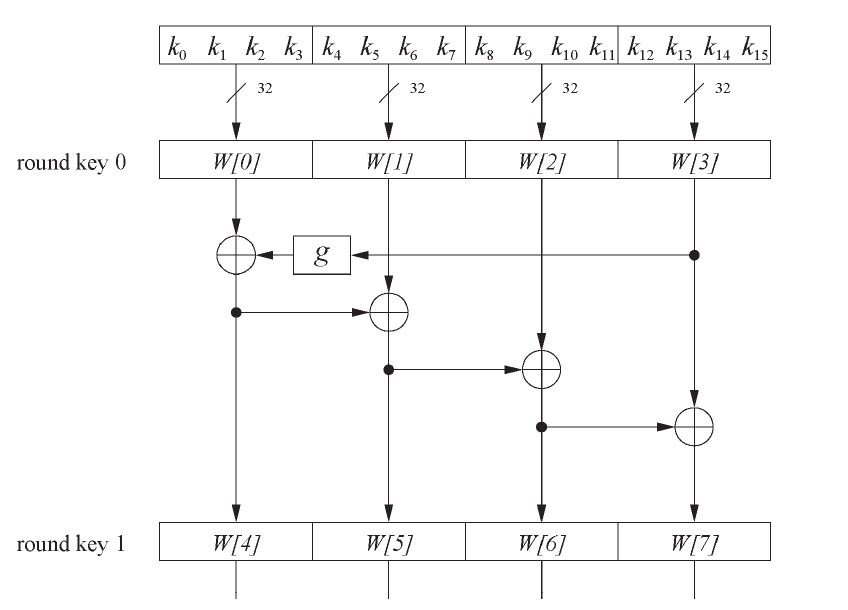
\includegraphics[scale=0.5]{key_sched_1_round.JPG} 
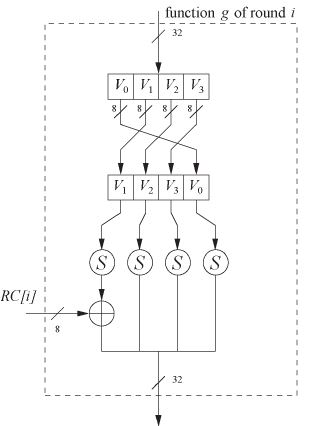
\includegraphics[scale=0.5]{aes_key_sched_function_g.JPG} \\
Die Funktion \textit{g} rotiert hierbei jeweils die Eingabebytes und führt sie durch eine nichtlineare S-Box. Am Ende dieses Verfahrens wird noch die Rundennummer mittels XOR dem linken Teilblock zugefügt. Das Ergebnis dieser Durchführung (W[4] bis W[7]) ist dann der Rundenschlüssel für die erste Runde. Dieses Verfahren wird wiederholt bis alle Rundenschlüssel entsprechend berechnet wurden. Die Anzahl der benötigten Rundenschlüssel und damit verbunden mit den benötigten Word-Blöcke erhöht sich mit der Erhöhung der Schlüssellänge von AES.

\subsubsection{Entschlüsselung}
Für die Entschlüsselung eines AES-Chiffretextes müssen alle Funktionen in umgekehrter Reihenfolge und umgekehrter Logik (Inverse Funktionen) ausgeführt werden. So hat man z. B. in der letzten Runde der Verschlüsselung die Funktion MixColumns nicht ausgeführt - so wird man in der ersten Runde der Entschlüsselung diese Funktion ebenfalls nicht ausführen. Darüber hinaus muss man für alle fixen Matrizen, die verwendet wurden eine inverse Matrix erstellen (S-Boxen, MixColumns-Matrix). Das Shifting in der Funktion ShiftRow erfolgt bei der Entschlüsselung dann entsprechend nach Rechts, anstatt nach Links wie bei der Entschlüsselung. Ausgenommen von der Umgekehrten Logik ist die Berechnung der Rundenschlüssel - da man in der ersten Runde der Entschlüsselung den letzten Rundenschlüssel benötigt, der bei der Verschlüsselung eingesetzt wurde, müssen zu Beginn der Entschlüsselung erstmals alle Rundenschlüssel berechnet werden um diese dann zu verwenden. Die Berechnung der Rundenschlüssel selbst ist identisch.



\subsection{ARC4}
RC4, oder auch ARC4 (Arcfour) genannt ist eine Stromverschlüsselung, wird also Bitweise ent- und verschlüsselt. %[Schneier, Seite 455]
Nach dem Aufdecken geheimer Informationen der NSA durch den Whistleblower Edward Snowden, hat der Kryptograph Jacob Appelbaum (Mitentwickler des Sicherheitsnetzwerkes Tor und Unterstützer von WikiLeaks) auf Twitter einen Post geteilt in dem er sagt, dass mit RC4 verschlüsselte Daten von der NSA in Echtzeit entschlüsselt werden können: "RC4 is broken in real time by the \#NSA - stop using it." %[https://twitter.com/ioerror/status/398059565947699200]
Diese Behauptung wird auch von Bruce Schneier (Experte für Kryptographie, Entwickler der Verfahren Blowfish und Twofish, Mitglied in mehreren Verbänden) in seinem offiziellen Blog als plausibel bestätigt: "Someone somewhere commented that the NSA's "groundbreaking cryptanalytic capabilities" could include a practical attack on RC4. I don't know one way or the other, but that's a good speculation." %[https://www.schneier.com/blog/archives/2013/09/the_nsa_is_brea.html] 
Darüber hinaus warnen verschiedene Seiten, wie Golem und Heise, die sich mit Informatik beschäftigen vor der Verwendung von RC4. %[ http://www.heise.de/newsticker/meldung/NSA-entschluesselt-Webserver-Daten-angeblich-in-Echtzeit-2041383.html, % http://www.golem.de/news/verschluesselung-was-noch-sicher-ist-1309-101457-2.html, http://www.theregister.co.uk/2013/09/06/nsa_cryptobreaking_bullrun_analysis/]
Selbst das Bundesamt für Sicherheit in der Informationstechnik (BSI) schreibt in einer technischen Richtlinie für Kryptographische Verfahren Anfang 2014: "Der Verschlüsselungsalgorithmus RC4 in TLS weist erhebliche Sicherheitsschwächen auf und darf nicht mehr eingesetzt werden." Das BSI gibt zusätzlich an, dass das Verschlüsselungsverfahren AES verwendet werden soll. %[https://www.bsi.bund.de/SharedDocs/Downloads/DE/BSI/Publikationen/TechnischeRichtlinien/TR02102/BSI-TR-02102-2_pdf.pdf?__blob=publicationFile]
Durch diese gezeigten Publikationen wird das Verfahren RC4 als unsicher angesehen und in dieser Arbeit nicht verwendet.


\subsection{Blowfish}
Blowfish ist eine Blockchiffrierung mit einer Blockgröße von 64 Bit. Wie auch bei DES und Triple-DES beschrieben ist diese Blockgröße für die heutigen Computer ungeeignet. Um diese Problem zu beheben hat der Erfinder des Verfahrens Bruce Schneier das Verfahren Twofish entwickelt, welches bei der Ausschreibung von AES auch unter den 5 Finalisten nominiert war. Es arbeitet auf einer Blockgröße von 128 Bit. Auch wenn es keine Beweisbaren belege für die Unsicherheit von Blowfish gibt, merkt Bruce Schneier in einem Interview an, dass man Twofish verwenden solle: "If people ask, I recommend Twofish instead." %http://www.computerworld.com.au/article/46254/bruce_almighty_schneier_preaches_security_linux_faithful/?pp=3
Aus der Analyse der Verfügbaren Kryptoverfahren, die in den verwendeten Android-Versionen angeboten werden ist Twofish noch nicht standardisiert enthalten. Durch die Validierung im späteren Kapitel bleibt offen, ob das Verfahren Blowfish in der Implementierung Einzug finden wird.

\subsubsection{Funktionsweise}
Die Vorgehensweise der Datenverschlüsselung von Blowfish beruht auf dem Feistel-Netzwerk. Hierbei wie der Block in 2 Hälften unterteilt, wobei die eine Teilhälfte immer durch eine Funktion verändert wird und die andere Teilhälfte in die nächste Runde weitergeben wird. Dabei wird bei jeder Runde beide Hälften miteinander vertauscht, sodass jede Teilhälfte alle 2 Runden der Funktion unterzogen wird. \\ \\
L$_{i}$ = R$_{i-1}$ \\
R$_{i}$ = L$_{i-1}$ $\oplus$ f(R$_{i-1}$, PK$_{i}$) \\ \\
In folgender Grafik wird das Verfahren von Blowfish und der Feistel-Struktur verdeutlicht dargestellt: \\ \\
%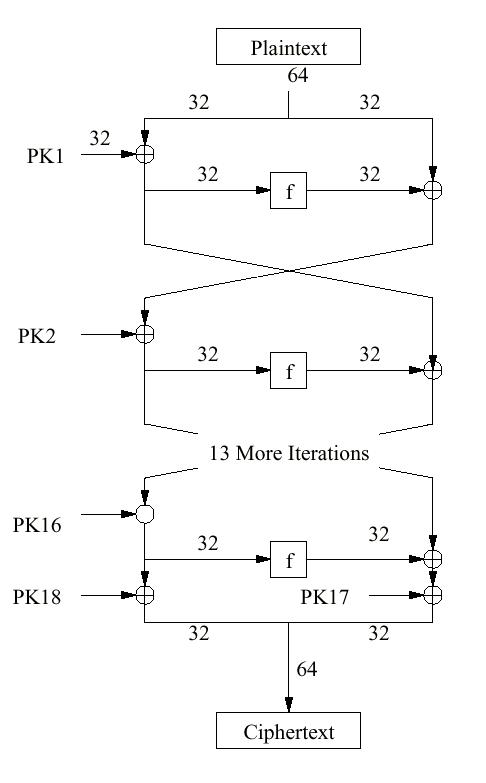
\includegraphics[scale=0.3]{blowfish_1.JPG} 


\begin{figure}[htbp]
\begin{minipage}[t]{4cm}
\vspace{0pt}
\centering
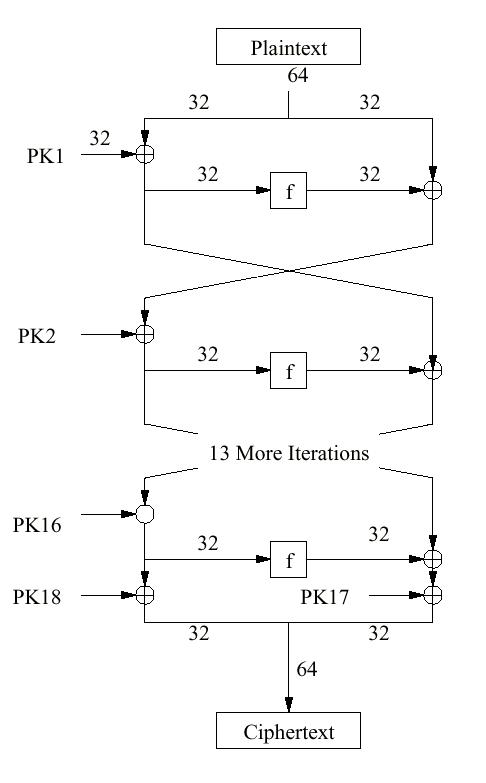
\includegraphics[scale=0.3]{blowfish_1.JPG}
\caption{Bild1}
\label{fig:Bild1}
\end{minipage}
\hfill
\begin{minipage}[t]{10cm}

Hierbei beschreibt PK$_{i}$ den Teilschlüssel der aktuellen Runde. Innerhalb der Funkion von Blowfish wird die 32 Bit große Teilhälfte in 4x8 Bit unterteile gesplittet und jeweils einer Substitution durch S-Boxen unterzogen. Im Gegensatz zu AES sind alle 4 S-Boxen in Blowfish verschieden. (Berechnung: siehe Teilschlüssel) Folgende Vorgehensweise wird innerhalb der Funktion durchgeführt: \\
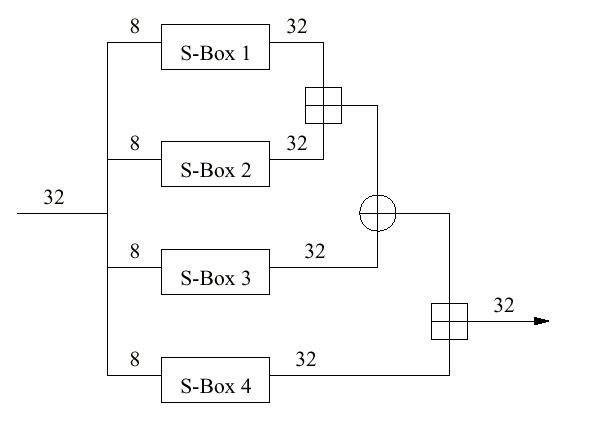
\includegraphics[scale=0.25]{blowfish_2.JPG} \\ % Schneier 1996, Seite 389f]
Das Ergebnis von S-Box 1 und S-Box 2 wird Addiert und Modulo 2$^{32}$ berechnet. Anschließend wird das Ergebnis mit dem Ergebnis von S-Box 3 XOR-Verknüpft und zum Schluss dessen Ergebnis mit dem Ergebnis aus S-Box 4 erneut addiert und Module 2$^{32}$ errechnet. Zusammenfassend ergibt das folgende Formel: \\ \\
F(x$_{L}$ = ((S$_{1,a}$ + S$_{2,b}$ mod 2$^{32}$) $\oplus$ S$_{3,c}$) + S$_{4,d}$ mod 2$^{32}$ \\ \\
\end{minipage}
\end{figure}
\subsubsection{Teilschlüssel}
Für die Generierung der Teilschlüsse, sowie der Erzeugung der S-Boxen existiert ein Algorithmus, der wie folgt vorgeht:
\begin{enumerate}
\item Das P-Array (Array der Größe 18, welches die Teilschlüssel mit je 32 Bit hält) und die vier S-Boxen werden der Reihe nach mit den Hexadezimalstellen von $\pi$ befüllt.
\item P$_{1}$ wird mit den ersten 32 Bit des Schlüssels XOR-Verknüpft, P$_{2}$ mit den zweiten. Ist das Schlüsselende erreicht, wird von vorne begonnen. Dieses Verfahren wird solange ausgeführt, bis alle 18 Felder des P-Arrays mit den Schlüsselbits XOR-Verknüpft sind.
\item Eine Zeichenkette bestehend aus Nullen wird in den Blowfish Algorithmus gegeben (Wichtig ist, dass hierbei bereits das geänderte P-Array verwendet wird)
\item Das Ergebnis der Verschlüsselung aus Punkt 3 wird als P$_{1}$ und P$_{2}$ verwendet.
\item Die Ausgabe von Punkt 3 wird erneut Verschlüsselt (Wieder mit dem geänderten P-Array)
\item Die Ausgabe von Punkt 5 wird zu P$_{2}$ und P$_{4}$.
\item Dieses Verfahren wird solange fortgesetzt, bis alle Elemente des P-Array, sowie der Reihe nach alle vier S-Boxen mit der Ausgabe des wechselnden Blowfish-Algorithmus ersetzt wurden.
\end{enumerate}
Bleibt der Schlüssel identisch, so kann die Anwendung die in 521 Iterationen errechneten Teilschlüssel speichern und muss diese nicht bei jeder Verschlüsselung neu errechnen.
Das hier gezeigte Verfahren zum Erstellen der Teilschlüssel wird auch Schlüsselexpansion genannt, da der Algorithmus nun auf insgesamt 4168 Bit Teilschlüsseln besteht. 
 
\section{Asymetrische Verfahren}
Im Gegensatz zu den bisher gezeigten Verschlüsselungsverfahren, ist der Ansatz bei Asymmetrischen Verfahren ein anderer. Bisher gab es einen geheimen Schlüssel, den man sowohl für die Verschlüsselung, als auch für die Entschlüsselung verwendete. Die Hauptaufgabe bei diesen Verfahren lag darin, den geheimen Schlüssel sicher von A nach B zur transportieren, ohne das ein eventueller Angreifer diesen mitlesen kann. Bei Asymmetrischen Verfahren ist der Grundgedanke derer, dass man jeweils zum Verschlüsseln einen Schlüssel besitzt als auch zum Entschlüsseln einen separaten Schlüssel. Der Schlüssel, welcher für die Verschlüsselung zuständig ist, wird Public Key genannt, da man ihn den Partnern öffentlich zuteilen kann. Das Pardon dazu ist der Private Schlüssel, der im eigenen Besitzt bleibt und nur dafür ist, die Verschlüsselte Nachricht wieder zu Dechiffrieren. Einer der Hauptaufgaben von Asymmetrischen Verfahren, oder auch Public-Key Verfahren genannnt, besteht darin 2 Schlüssel zu finden, zwar jeweils für die Verschlüsselung und Entschlüsselung zu gebrauchtn sind, aus denen man aber den jeweils anderen Schlüsselteil nicht errechnen kann. Der Grundgedanke dieses Verfahrens stammt von Whitfield Diffie und Martin Hellman, die hierzu 1976 ein Konzept auf der \textit{National Computer Conference} vorstellen. 

\subsection{RSA}
RSA, nach den Erfindern Rivest, Shamir und Adleman benannt ist, ist eines der oben beschriebenen Asymmetrischen Kryptoverfahren. Die Sicherheit von RSA beruht auf dem Problem der Primfaktorzerlegung - d. h. es ist schwierig, aus einem gegebenem Faktor 2er Primzahlen, diese zurück zu rechnen. \\
Das Erstellen der Schlüssel wird wie folgt ausgeführt: \\
\begin{enumerate}
\item wähle 2 große Primzahlen p und q
\item berechne n = p * q
\item berechne phi(n) = (p-1) * (q-1)
\item wähle ein e für das gilt e $\in$ \{1,2,...,phi(n)-1\} und ggT(e, phi(n)) = 1
\item berechne d, sodass gilt d * e $\equiv$ 1 mod phi(n)
\item Öffentlicher Schlüssel = (n,e) , Privater Schlüssel = d \\
\end{enumerate} 
Nach der Berechnung kann der öffentliche Schlüssel (n,e) frei zugänglich gemacht werden. Dieser Schlüssel wird verwendet um Nachrichten zu Verschlüsseln, oder eine Nachricht zu signieren (siehe Digitale Signaturen). Zum Entschlüsseln des entsprechenden Chiffretextes wird der private Schlüssel d benötigt. Die Werte p, q, phi(n) werden nicht mehr benötigt, dürfen jedoch auch nicht frei zugänglich gemcht werden, da mit diesen die Berechnung des privaten Schlüssels erfolgen kann. Zum Chiffrieren und Dechiffrieren einer Nachricht werden folgende mathematische Funktionen angewandt, wobei M = Message und C = Chiffrat bedeutet: \\
\begin{itemize}
\item C = M$^{e}$ mod n
\item M = C$^{d}$ mod n \\
\end{itemize}
Die Schlüssellänge des Verfahrens RSA ist variabel zwischen 512 und 2048 zu wählen, wobei sie die Bitlänge der berechneten Zahl n beschreibt. Zu beachten ist außerdem, dass es lediglich möglich ist Werte zu Verschlüsseln die im Bereich M $\in$ \{0, ... , n-1\} liegen. Um dennoch größere Nachrichten zu verschlüsseln, teilt man den Klartext in Blöcke auf und verschlüsselt diese einzeln mit dem Verfahren. Zur Entschlüsselung werden nach der Dechiffrierung die entsprechenden Blöcke wieder aneinandergehängt. \\
Die Geschwindigkeit des Verfahrens hängt stark von der Wahl der Exponenten ab. Wählt man den öffentlichen Exponent e relativ klein, so wird die Verschlüsselung entsprechend schneller, hingegen ein großer privater Schlüssel d die Entschlüsselung entsprechend längere Zeit in Anspruch nimmt. Darüber hinaus ist es wichtig um die Performance von RSA zu steigern eine Möglichkeit zu finden, große Exponenten schnell zu errechnen. Hierbei kommt das Square- and Multiply Verfahren zum Einsatz.
 %https://www.youtube.com/watch?v=QSlWzKNbKrU

\subsection{ElGamal}
ElGamal ist, wie auch RSA, ein Asymmetrisches Verfahren - d. h. es gibt einen öffentlichen- und einen privaten Schlüssel. Die Sicherheit des Verfahrens besteht in der Schwierigkeit diskrete Logarithmen über einen endlichen Körper zu berechnen. \\
Um ein Schlüsselpaar zu erzeugen wählt man eine Primzahl p und zwei Zufallszahlen g und x, welche kleiner als p sind und berechnet: \\ \\
y = g$^{x}$ mod p \\ \\
Der öffentliche Schlüssel ist y, g und p - der private Schlüssel ist x. Um eine Nachricht zu verschlüsseln wählt man ein zufälliges k, welches relativ prim zu p-1 ist ( 1 = ggT(k,p-1) ) und berechnet die Verschlüsselung wie folgt: \\ \\
a = g$^{k}$ mod p \\
b = y$^{k}$ M mod p \\ \\
wobei a und b den Chiffretext bildet, welcher doppelt so lang ist wie der Klartext. Die Entschlüsselung des Chiffretextes erfolgt dann durch: \\ \\
M = b/a$^{x}$ mod p \\


\subsection{Digitale Signatur}
Digitalte Signaturen, oder auch elektronische Signaturen sind in der Lage die, im Grundlagen Kryptologie Kapitel, gezeigten Anforderungen (Authentizität, Integrität und Verbindlichkeit) zu erfüllen. Zur Durchführung digitaler Signatur werden asymmetrische Verschlüsselungsverfahren verwendet (z. B. RSA oder ElGamal). Im folgenden Beispiel soll erläutert werden, wie das Verfahren der elektronischen Signatur anzuwenden ist. Angenommen es gibt 2 Teilnehmer die sich Daten senden wollen (in dem Fall Alice und Bob) und beide Parteien verfügen über den jeweils öffentlichen Schlüssel des Gegenübers. \\
Alice signiert das Dokument mit ihrem privaten Schlüssel K$_{PrivA}$ (aus Perfomancegründen wird lediglich der Hash-Wert (siehe Kapitel Hash-Funktionen) der Nachricht signiert) und verschlüsselt dann die Nachricht und Signatur mit dem öffentlichen Schlüssel von Bob K$_{PubB}$. \\ \\
sig =  E(K$_{privA}$, Hash(M)) \\
C = E(K$_{PubB}$, M + sig)) \\ \\
Der Chiffretext C wird dann zu Bob übertragen, der im ersten Schritt die Nachricht mit seinem privaten Schlüssel K$_{privB}$ entschlüsselt. Anschließend entschlüsselt er die digitale Signatur mit dem öffentlichen Schlüssel von Alice K$_{PubA}$. Bob errechnet nun aus der bereits entschlüsselten Nachricht den Hash-Wert und prüft den mit den Hash-Wert aus der Signatur - stimmen beide Werte überein ist die Nachricht verifiziert. \\ \\
M, sig = D(K$_{PrivB}$, C) \\
AliceHash(M) = D(K$_{PubA}$, sig) \\
AliceHash(M) ?= Hash(M) \\ \\
Unter der Voraussetzung, dass beide Parteien sicher sind den öffentlichen Schlüssel des gewünschten Partners zu besitzen sorgt dieses Verfahren dafür, dass Bob nach dem Verifizieren der Nachricht zum einen sicher sein kann, dass nur Alice (als alleinige Besitzerin des privaten Schlüssels) die Nachricht unterschrieben hat (Authentifizierung und Verbindlichkeit), zum anderen kann er aufgrund des Hash-Wertes der Nachricht sicher sein, dass die Nachricht bei der Übertragung nicht verfälscht wurde (Integrität).



\section{Hash-Funktionen}
Hash-Funktionen sind mathematische Einweg-Funktionen - das bedeutet, dass ein Wert h = H(M) leicht erzeugt werden kann, jedoch nicht aus h wieder M - es existiert keine Umkehrfunktion. Darüber hinaus ist es praktisch nicht möglich verschiedene Eingabewerte M1, M2, ... zu finden, die den selben Ausgabewert erzeugen H(M) = H(M1). Da Hash-Funktionen eine Nachricht beliebiger Länge auf einer Nachricht fester Länge abbilden ist eine Abbildung auf einen identischen Hash-Wert nicht auszuschließen. Es muss also eine Hash-Größe gewählt werden, sodass es praktisch unmöglich ist alle möglichen Hash-Werte zu berechnen und zu speichern. Ist die Hash-Größe lediglich 64 Bit lang, so gibt es 2$^{64}$ Möglichkeiten einen Hash-Wert. Dem Angreifer reichen jedoch 2$^{32}$ Nachrichten M und den dazugehörigen Hash-Wert h = H(M), sodass die Wahrscheinlichkeit für eine Kollision größer als 0,5 ist. Diese Erkenntnis beruht auf dem Geburtstags-Paradoxon, welches besagt, dass lediglich 23 Personen in einem Raum genügen, um mit einer Wahrscheinlichkeit größer als 0,5, 2 davon zu finden, die am selben Tag Geburtstag haben. Diese Logik lässt sich auch auf Hash-Funktionen abbilden und kann somit die Komplexität, eine Kollision mit über 50\% Wahrscheinlichkeit zu finden, von 2$^{k}$ auf k * 2$^{k/2}$ reduzieren.

\subsection{MD5 \& SHA1}
Wie beschrieben sollen Hash-Funktionen eine Größenordnung besitzen, die es heutigen Systemen schwierig macht Kollisionen zu errechnen und zu speichern. MD5 arbeitet mit einer Größe von 128bit und es ist möglich mit nur 2$^{64}$ Schritten eine Kollision zu entdecken (Geburtstags-Paradoxon). Ähnliches Problem zeigt sich bei der Verwendung von SHA1, welches eine Hashwert-Größe von 160 bit hat, also 2$^{80}$ Schritte für eine Kollision. Beide Größenordnung reichen für heutige Systeme nicht aus und sollten deshalb nicht verwendet werden.

\subsection{SHA224, SHA256, SHA384, SHA512}
Alle 4 Hash-Funktionen gehören zur SHA2-Familie und sind von der Vorgehensweise zur Berechnung des Hash-Wertes identisch. Unterschieden sind zwischen SHA256 und SHA512 die Blockgröße (512 Bit, 1024 Bit), Die Anzahl der Wörter (16x32Bit Wörter, 16x64Bit Wörter), sowie die Anzahl der Konstanten (64 Konsanten, 80 Konstanten). Bei den Verfahren SHA224, sowie SHA384 wird jeweils das größere Hash-Verfahren komplett berechnet und die letzten entsprechenden Bits weggelassen. Da sich die Verfahren von Ihrer Funktionsweise nicht unterscheiden, wird hier lediglich SHA256 näher erklärt.  \\ \\
Zu Beginn werden 8 Blöcke je 32 Bit (256 Bit = Hash-Größe) initialisiert (Nachkommastellen der Wurzeln der ersten 8 Primzahlen), sie erhalten die Bezeichnungen a - h. Auf ihnen finden mathematische Funktionen statt. Ausserdem werden 64 Blöcke je 32 Bit mit Rundenkonstanten (Bestimmt aus den Kubikwurzeln der ersten 64 Primzahlen), sie erhalten die Bezeichnung k[i].
Der Klartext wird in 512 Bit große Blöcke unterteilt und, falls erforderlich, am Ende aufgefüllt. Jeder Block wird nun in 16 x 32 Bit Worte aufgesplittet . Diese 16 Worte werden anschließend auf 64 Worte expandiert. Für jedes dieser 64 Worte (im folgenden w[i]) finden nun folgende mathematischen Funktionen statt: (i ist hierbei die Zählervariable der Wörter) \\ \\
S1 := (e $\gg$ 6) $\oplus$ (e $\gg$ 11) $\oplus$ (e $\gg$ 25) \\
ch := (e $\land$ f) $\oplus$ ($\lnot$ e $\land$ g) \\
temp1 := h + S1 + ch + k[i] + w[i]\\
S0 := (a $\gg$ 2) $\oplus$ (a $\gg$ 13) $\oplus$ (a $\gg$ 22) \\
maj := (a $\land$ b) $\oplus$ (a $\land$ c) $\oplus$ (b $\land$ c) \\
temp2 := S0 + maj \\ \\
Nach dieser Berechnung findet eine Verschiebung der Variablen statt (h=g ; g=f ; f=e ; e=d+temp1 ; d=c ; c=b ; b=a ; a=temp1+temp2). \\
Nachdem die oben beschriebene Berechnung für alle 64 Runden durchgeführt wurde, werden die entsprechenden Werte (a-h) miteinander konkateniert und ergeben somit den Hash-Wert.

\subsection{Message Authentification Code}
Hash-Funktionen an sich bieten lediglich die Sicherheit der Integrität der Daten, also dass die Daten beim Empfänger unverändert angekommen sind. Über den Ursprung der Daten, also die Authentizität, kann eine Hash-Funktion keine Sicherheit gewährleisten. Um dieses Problem zu beheben gibt es das MAC-Verfahren (Message Authentification Code). MAC-Funktionen verwenden zum errechnen eines Hash-Wertes zusätzlich einen geheimen Schlüssel der beiden Parteien vor der Kommunikation bekannt sein muss. Wird dem Dokument entsprechend ein MAC-Wert angefügt so muss der Empfänger die selbe MAC-Funktion auf das Dokument anwenden und prüfen ob beide MAC-Werte (der selbst errechnete und der zugesandte) übereinstimmen - ist dies der Fall, so ist die Authentizität gewährleistet (sofern sichergestellt ist, dass der Schlüssel geheimgehalten wurde). Dieses Verfahren ist jedoch nicht in der Lage Verbindlichkeit zu gewährleisten (einem dritten glaubwürdig zu machen, wer der Absender ist), da auch der Empfänger in der Lage ist, den entsprechenden MAC zu berechnen. 


\section{Schlüsselvereinbarung} 
Das Hauptproblem für alle Kryptografischen Ver- und Entschlüsselungsverfahren ist die Vereinbarung eines gemeinsamen Schlüssels. Selbst bei Asymmetrischen Verfahren ist nicht sichergestellt, dass durch einen Man-in-the-middle Angriff ein potentieller Angreifer, seinen eigenen Public-Key in das System schleust und somit über den dazugehörigen Privaten Schlüssel verfügt. Verschiedene Verfahren sollen es ermöglich einen Schlüssel auszutauschen, ohne das ein Angreifer diesen auch erhält.

\subsection{Diffie Hellmann}
Dieses Verfahren beruht auf einfacher mathematischer Potenzierung und Modulo-Rechnung, für den Angreifer besteht jedoch das Problem der diskreten Logarithmen in endlichen Körpern (siehe RSA-Verfahren). Das Problem dieses Verfahrens ist, dass es gegen Man in the middle Agriffe nicht geschützt ist, da ein potentieller Angreifer seine eigenen Potenzen und Modulo-Werte in das System schleusen kann und aufgrund dessen beide Parteien den privaten Schlüssel berechnen. [Schneier 587, Ferguson 211]

\subsection{Direkte Vereinbarung}
\subsubsection{QR-Code}
\subsubsection{PGP-Server}
%\section{Authentifizierung}
%\subsection{Zwei-Faktor-Authentifizierung}
	% TODO: Erklärung: http://de.wikipedia.org/wiki/Zwei-Faktor-Authentifizierung (need Quelle)


%% ------------------------ VALIDIERUNG --------------------- %%
\chapter{Validierung}
	% TODO: Erläuterung des Testgerätes & der Punkte auf die getestet werden soll!
	% aufzeigen der Notwendigkeit dieser Validierung
Bei der Validierung soll gezeigt werden ob die im vorigen Kapitel als sicher angesehen Verfahren auch auf heutigen Android-Geräten zum Einsatz kommen können. Hierbei sollen die Verfahren im Bezug auf ihre Schlüssellänge, sowie die Dateigröße validiert werden. Die Validierung soll in Bezug auf Geschwindigkeit bzw. Dauer des Verfahrens, Akkuverbrauch und Wärmeentwicklung durchgeführt werden. 


\section{Verschlüsselungsverfahren}
\section{Hashfunktionen}

%% ------------------------ IMPLEMENTIERUNG ---------------- %%
\chapter{Implementierung}
\section{Entwurf}

%% ----------------------------- TEST -------------------------- %%
\chapter{Test}
\section{Validierung}
\section{Testverfahren}

%% -------------------------- ZUSAMMENFASSUNG -------------- %%
\chapter{Zusammenfassung und Ausblick}
\section{Zusammenfassung}
\section{Ausblick}
	
%--------------------------------------------------------------------
% -----------------------ENDE ------------------------------------
%------------------------------------------------------------------


%% --------------------------- BIBLIO --------------------------------%%
%\label{Bibliography}s

%\lhead{\emph{Bibliography}} % Change the page header to say "Bibliography"

%\bibliographystyle{unsrtnat} % Use the "unsrtnat" BibTeX style for formatting the Bibliography

%\bibliography{Bibliography} % The references (bibliography) information are stored in the file named "Bibliography.bib"

\printindex

%Glossar
%Literatur
%Diagramme
%Tabellen
%eigenständigkeitsverklärung

%% ---------------------------------- ANHANG --------------------------- %%
	%TODO: Algorithmen 411 und 322.

\end{document}